\documentclass[a4paper]{article}
\renewcommand{\baselinestretch}{1.1}
\usepackage[utf8]{inputenc}
\usepackage[english]{babel}
\usepackage[T1]{fontenc}
\usepackage{graphicx}
\usepackage{hyperref}
\hypersetup{
	colorlinks = true,	
}
\usepackage{prettyref}
\newrefformat{fig}{A.\ref{#1}}
\usepackage{amsmath}
\usepackage{amssymb}
\usepackage{caption}
\usepackage[output-decimal-marker={,}]{siunitx}
\usepackage{booktabs}
\usepackage{subfig}
\usepackage{float}
\usepackage{geometry}
\usepackage{multicol}
\usepackage{listings}
\newenvironment{Figure}
	{\par\medskip\noindent\minipage{\linewidth}}
	{\endminipage\par\medskip}
\geometry{
	a4paper,
	total={170mm,257mm},
	left=20mm,
	top=20mm,
}

\title{Extraction of Spectra and its Application to an Atmosphere Problem}
\author{Alessandro Lattanzi}
\date{\today}

\begin{document}
	\maketitle
	
	\section{Introduction}
	The goal of this analysis is to extract a spectrum using a spectrograph. This is then used to reconstruct atmospheric transmission and CCD response function from a series of measurements.\\
	In order to extract a spectrum the image must first be cleaned by applying flat and dark, fine-aligned, and finally calibrated using a lamp.\\
	To reconstruct atmospheric transmission and CCD response two spectra of Sirius were taken with the "Alpy 600" spectrograph and the standard spectrum of Vega was used as a calibration.\\
	\newline
	\textit{The full commented code and source material is available at \url{https://github.com/alelatt/Osservativa}}
	
	\vspace{0.035\textheight}
	
	\section{Spectrum Extraction}
	\begin{multicols}{2}
		The following describes the procedure used to extract a spectrum from an image.\\
		At the end of the extraction procedure the user can save a calibration file with all the relevant parameters, so that the next time the spectrum needs to be extracted no user input is necessary (if the user chooses to use the saved calibration).
		
		\subsection{Image Correction}
			At the beginning of the night five flat frames and two dark frames were taken. Master flat and master dark were obtained by averaging these images.\\
			It's worth noting that the two dark frames have an exposure time of 20s, while the dark frames have an exposure of 10s. Some of the images have an exposure time different from that of the dark frames, thus, for these images, the master dark needs to be rescaled to the correct exposure time. This clearly isn't a problem when applying the flat since its always scaled to have mean = 1.
			Master dark and master flat are thus applied to the science frame and the lamp frame.\\
		
		\subsection{Fine-Rotation}
			This procedure and the next ones are managed interactively by the user.\\
			The corrected image is shown to the user, who is then asked to select a rectangular window inside which the spectrum lies.\\
			100 equally-spaced points in the dispersion direction are picked inside the given range and the peak in the cross-dispersion is found together with an averaged (before and after the peak) Half-Width-Half-Maximum as an "error" on the position of the peak.
			
			\begin{Figure}
				\centering
				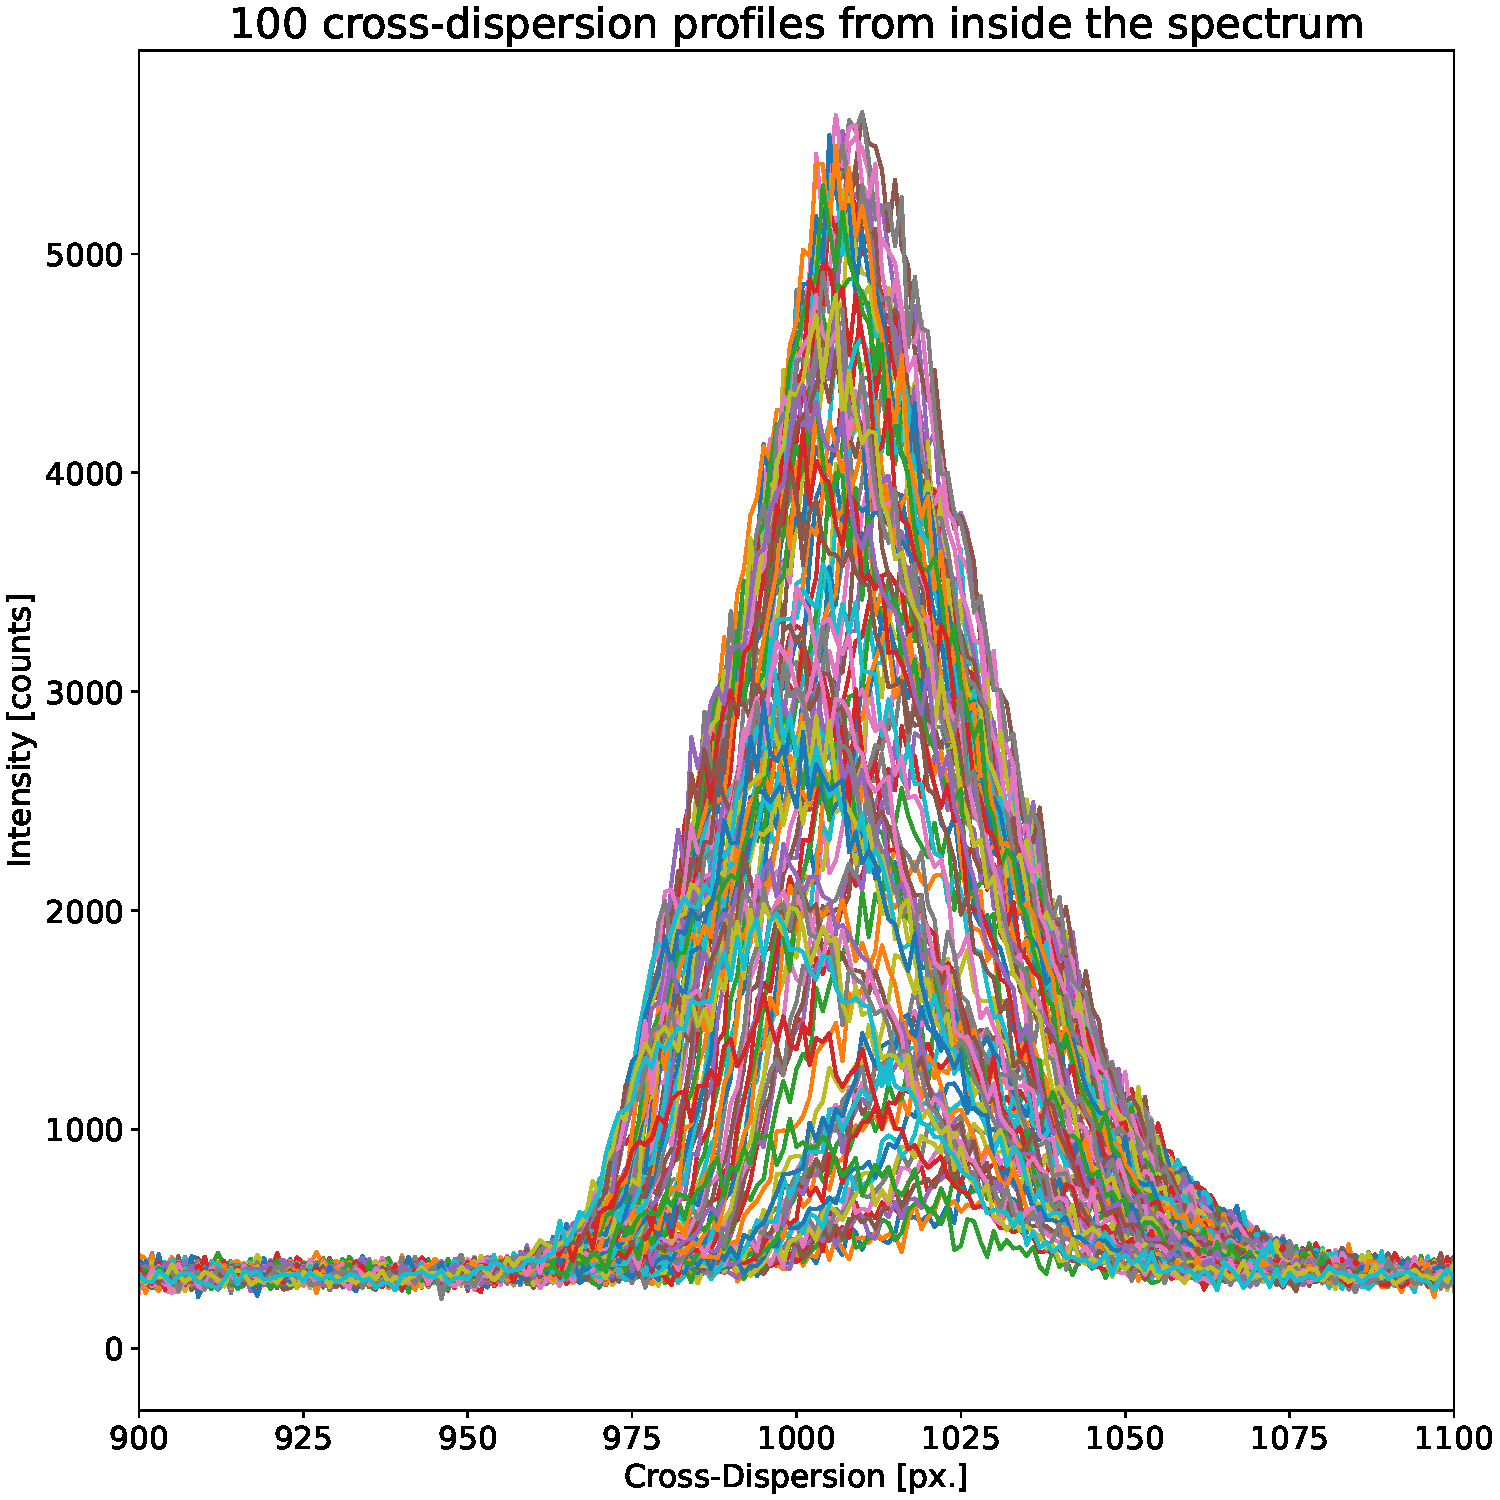
\includegraphics[width=0.98\linewidth]{Rot_ang_profiles.pdf}
				\captionof{figure}{Cross-dispersion profiles at 100 points}
				\label{fig:rot_prof}
			\end{Figure}
		
			A line is then fitted through these points and its slope is used to find the rotation angle of the spectrum.
			\begin{Figure}
				\centering
				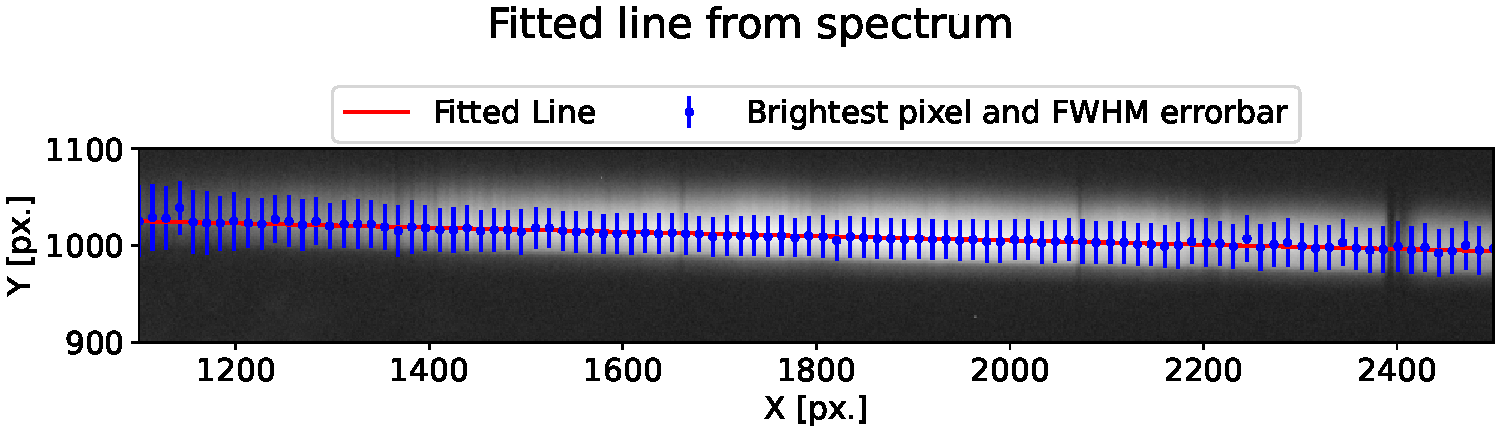
\includegraphics[width=\linewidth]{Rot_ang_fit.pdf}
				\captionof{figure}{Linear fit over the points}
				\label{fig:rot_fit}
			\end{Figure}
			
			The image can now be rotated. The lamp is also rotated in order to take the exact same window later on when extracting the lamp spectrum to calibrate the spectrum.\\
		
		\subsection{Spectrum Extraction}
			The user is once more shown the now rotated image and asked to select a window inside which the spectrum is extracted.\\
			This procedure is as follows: first the user has to choose the lower and upper bounds in the dispersion direction, then the user has to choose a center-line for the spectrum and finally a cross-dispersion half-width over which the spectrum is averaged.\\
			Before each step the image is shown with the bounds chosen at the previous step in order to facilitate the next choice. At the end of the operation another window can be chosen if the first isn't satisfactory.\\
			
			\begin{Figure}
				\centering
				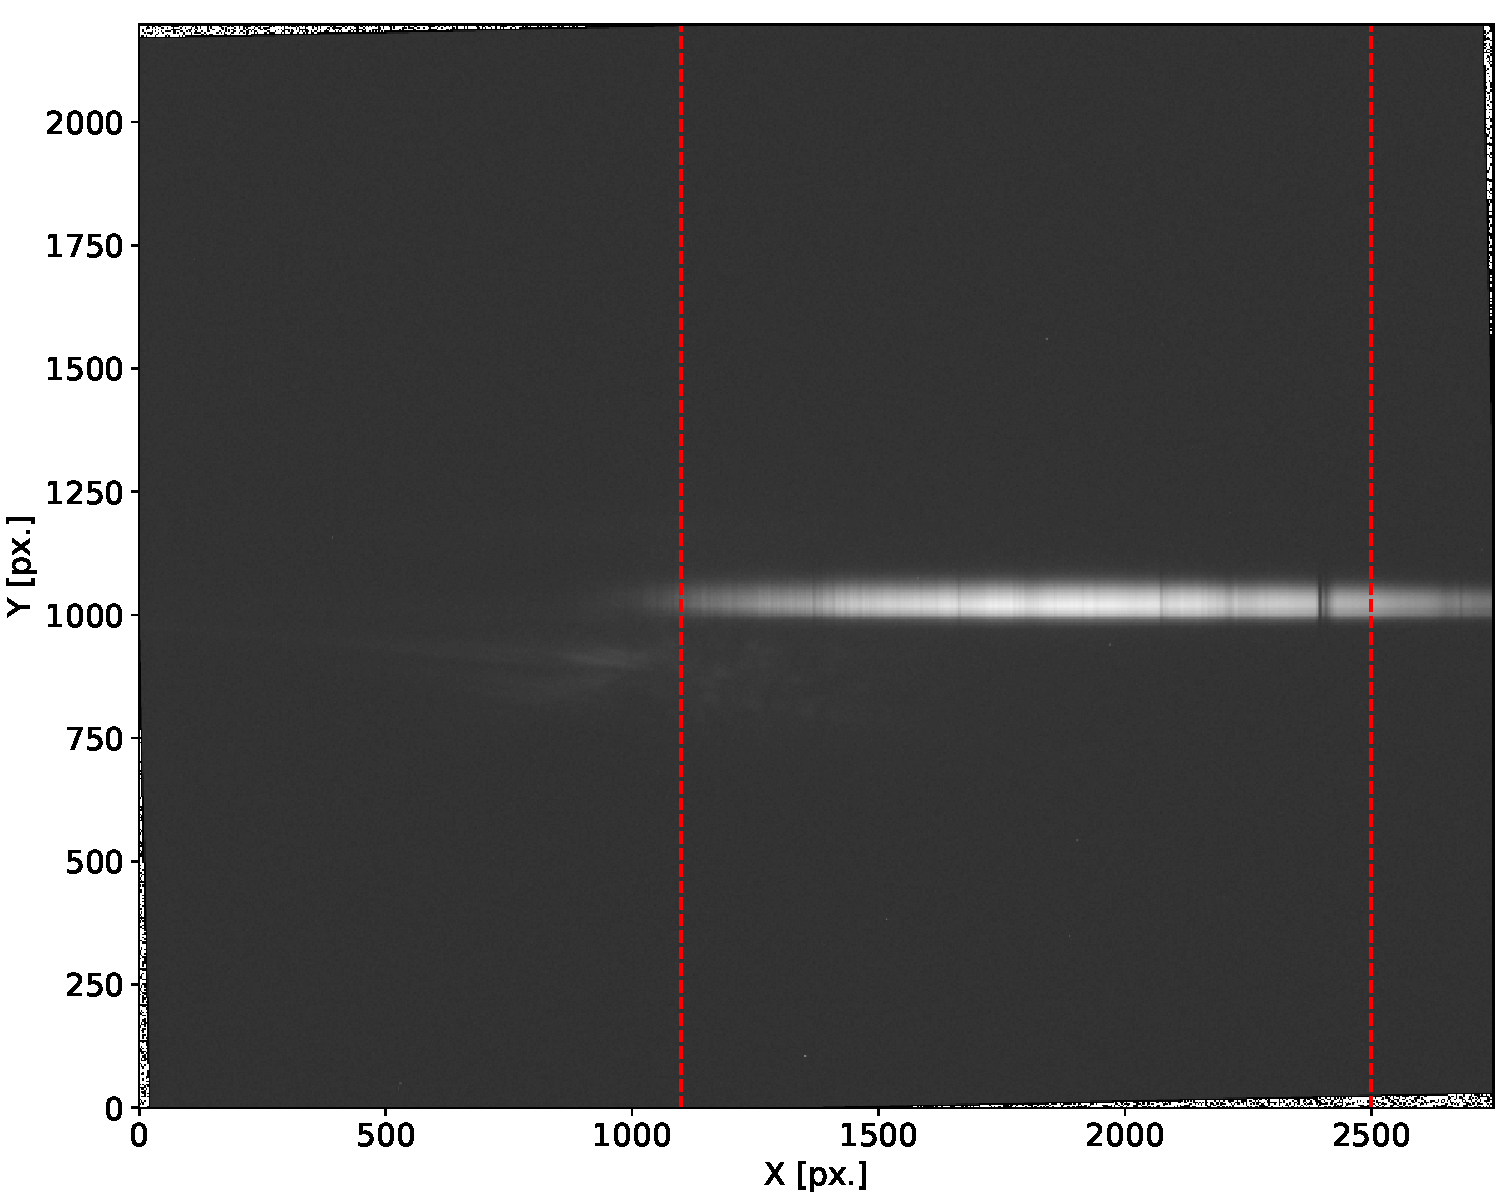
\includegraphics[width=\linewidth]{Extr_step1.pdf}
				\captionof{figure}{Dispersion direction bounds}
				\label{fig:extr1}
			\end{Figure}
			\begin{Figure}
				\centering
				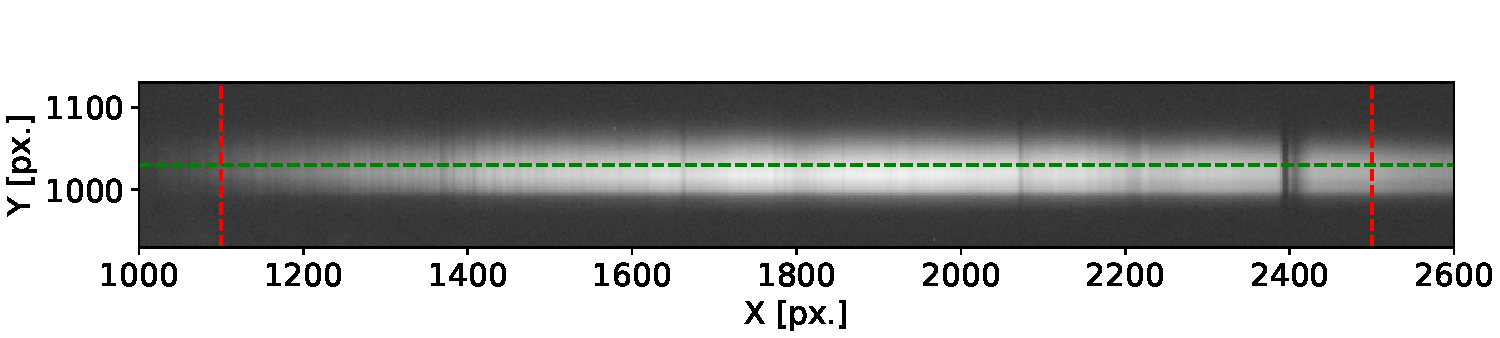
\includegraphics[width=\linewidth]{Extr_step2.pdf}
				\captionof{figure}{Center line}
				\label{fig:extr2}
			\end{Figure}
			\begin{Figure}
				\centering
				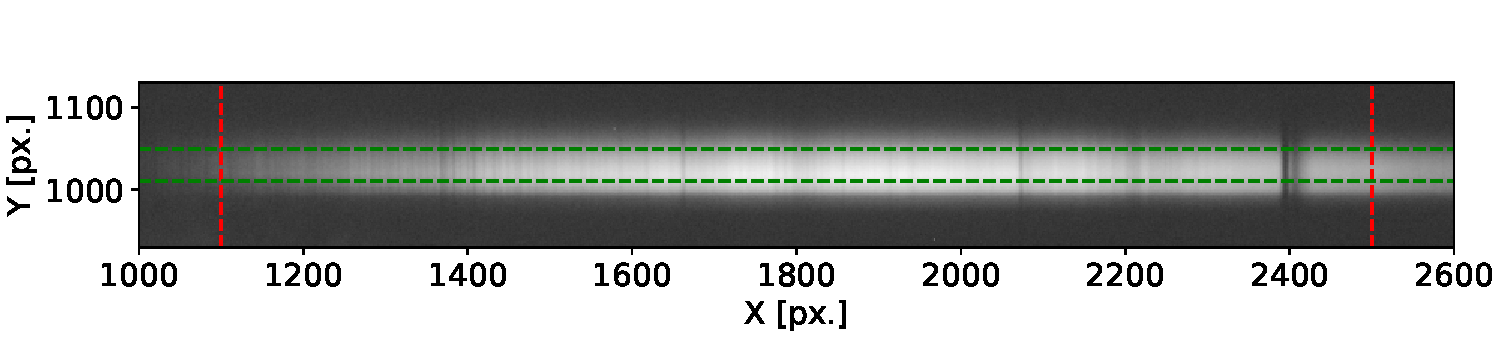
\includegraphics[width=\linewidth]{Extr_step3.pdf}
				\captionof{figure}{Cross dispersion width and final window}
				\label{fig:extr3}
			\end{Figure}
			
			During this operation the user should make sure to select a portion of the image that contains only the spectrum in the cross-dispersion direction so as not contaminate the average with background.\\
			
			The lamp frame is extracted and averaged on the exact same section of the image.\\
			
		\subsection{Spectrum Calibration}
			Having now extracted both spectrum and lamp the user is shown the extracted lamp spectrum and an image containing the lines generated by the Ne/Ar/H lamp and the relative wavelengths.\\
			\begin{Figure}
				\centering
				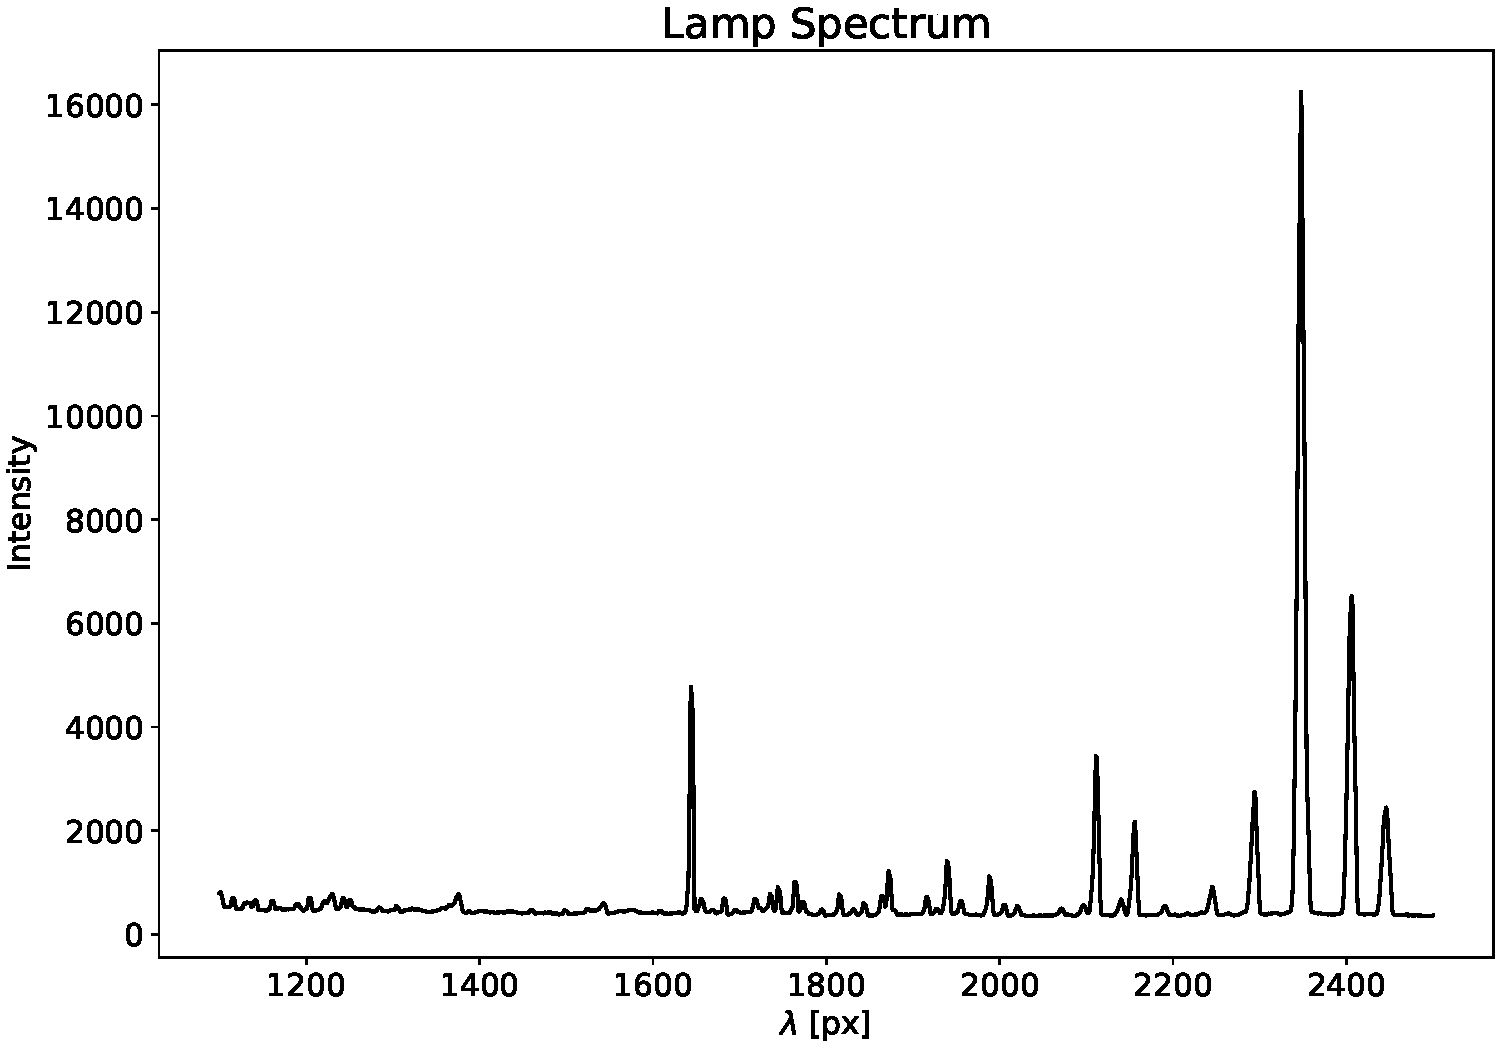
\includegraphics[width=\linewidth]{Lamp_spectr.pdf}
				\captionof{figure}{Lamp spectrum}
				\label{fig:lamp_s}
			\end{Figure}
			\begin{Figure}
				\centering
				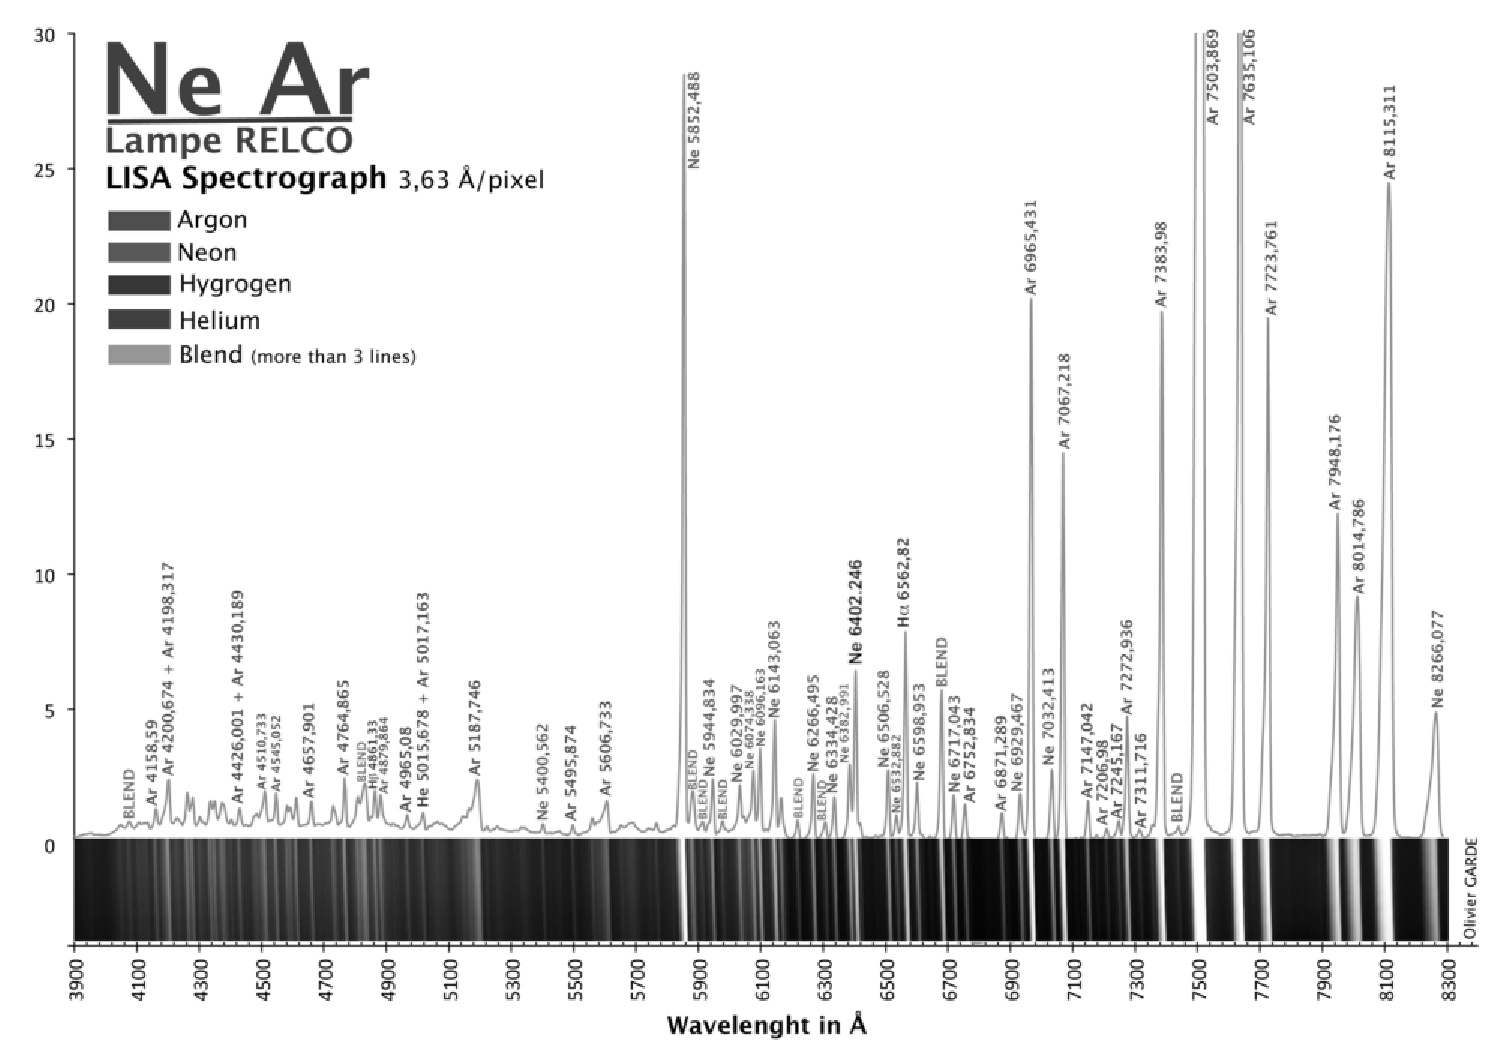
\includegraphics[width=\linewidth]{Lamp_image.pdf}
				\captionof{figure}{Lamp reference image}
				\label{fig:lamp_i}
			\end{Figure}
			The user has to input the dispersion position (in pixel) and the wavelength of as many lines as needed using the console. These points are then fitted using a second degree polynomial to get the conversion between pixels and wavelength.\\
			Since the rotation angle is ever so slightly different between spectra, the polynomial coefficients are not exactly the same between spectra.\\
			
			The choice to use a second degree polynomial was taken after verifying that using anything more than a third degree polynomial results in overfitting and a linear polynomial is not sufficient. Between a third degree polynomial and a second degree one, the second degree polynomial performed better in a series of tests.\\
		
		\subsection{Airmass}
			The user is also asked to input the observed object's ICRS coordinates, needed, together with the observation date and time present in the \textit{fits} file, to compute the airmass at time of observation.\\
		
	\end{multicols}

	\vspace{0.035\textheight}

	\section{An application: Atmospheric transmittance and CCD response}
	\begin{multicols}{2}
		\subsection{Description of the exercise}
			The goal of this exercise is to find the atmospheric and CCD response functions starting from two spectroscopic observations of Sirius taken the same night at different airmasses.\\
			In order to achieve this the atmospheric transmittance is first recovered using the two Sirius spectra. Using Vega as a close enough match for Sirius, the idea is to use the standard spectrum of Vega together with the observed spectra of Sirius to get the total response function (atmosphere and CCD).\\
			From the total response function and the atmospheric transmittance, the CCD response can also be computed.\\
			
		\subsection{Preparatory steps}
			The spectra from the two Sirius observations are extracted as detailed in Section 2.\\
			
			The standard Vega spectrum is available at \url{https://ftp.eso.org/pub/usg/standards/hststan/}.\\
			It is immediately worth noting that by using the absolute spectrum of Vega we get dimensional quantities for the total response function and, consequently, for the CCD response (since the atmospheric transmittance is dimensionless).\\
			
			The three spectra are binned to 50 \si{\angstrom} centered around the same wavelengths in order to operate on them.
		
		\subsection{Atmospheric Transmittance}
			Let $N_i(t_{exp,i}, a_i)$ be the measured Sirius spectra, with $i = 1,2$, $t_{exp,i}$ the relative exposure time and $a_i$ the airmass.\\
			
			In principle we can write (omitting frequency dependence everywhere):
			\begin{equation}
				N(t_{exp}, a) = I \cdot R(t_{exp}, a) = I \cdot T(a) \cdot S(t_{exp})
			\end{equation}
			\begin{equation}
				T(a) = (T_0)^a = (e^{-\tau})^a
			\end{equation}
			\begin{equation}
				S(t_{exp}) = S_0 \cdot t_{exp}
			\end{equation}
			where $T(a)$ is the atmospheric transmittance at airmass a, $T_0 = e^{-\tau}$ the standard transmittance at $a = 1$, $S(t_{exp})$ is the instrument response function which, supposing that the response is time independent, can be written as above with a term $S_0$ only dependent on the CCD characteristics.\\
			
			It was noticed that this description doesn't totally fit the observations and an additional multiplicative term $A$ independent of frequency and time was added such that $N_i(t_{exp,i}, a_i) = I \cdot R(t_{exp,i}, a_i) \cdot A_i$.\\
			This term is defined in the simplest way possible, even though all the effects that it might encompass will be airmass and frequency dependent. These effects might be curvature and the different absorption it gives with respect to the plane parallel approximation, other atmospheric effects that come into play since the two measurements were taken an hour apart in not perfect sky conditions, different background illuminations and so on.\\
			The presence of this additional term will give problems later on when looking for an analytical solution.\\
			
			First we need to find the optical depth $\tau_{\lambda}$.\\
			We have:
			\begin{equation}
					\frac{N_1}{N_2} = e^{(a_2 - a_1) \tau_{\lambda}} \frac{t_{exp,1} \cdot A_1}{t_{exp,2} \cdot A_2}
			\end{equation}
			from which
			\begin{equation}
				\frac{1}{a_2 - a_1}\ln\left(\frac{N_1}{N_2}\right) = \tau_{\lambda} - \frac{1}{a_2 - a_1}\ln\left(\frac{t_{exp,2} \cdot A_2}{t_{exp,1} \cdot A_1}\right)
			\end{equation}
			\newline
			If $\tau_{\lambda}$ can be modeled as an exponential we can fit 
			\begin{equation*}
				\tau_{\lambda}^{'} = \exp(\alpha (\lambda - \beta)) + c
			\end{equation*}
			with $\tau_{\lambda}^{'} = \frac{1}{a_2 - a_1}\ln\left(\frac{N_1}{N_2}\right)$.
			\newline
			\newline
			We can thus derive $\tau_{\lambda}$ and $T_0 = e^{-\tau_{\lambda}}$.\\
			Rayleigh scattering optical depth is used as reference\footnote{From Noll et al. (2012), available at  \url{https://www.aanda.org/articles/aa/full_html/2012/07/aa19040-12/aa19040-12.html}}.\\
			\begin{Figure}
				\centering
				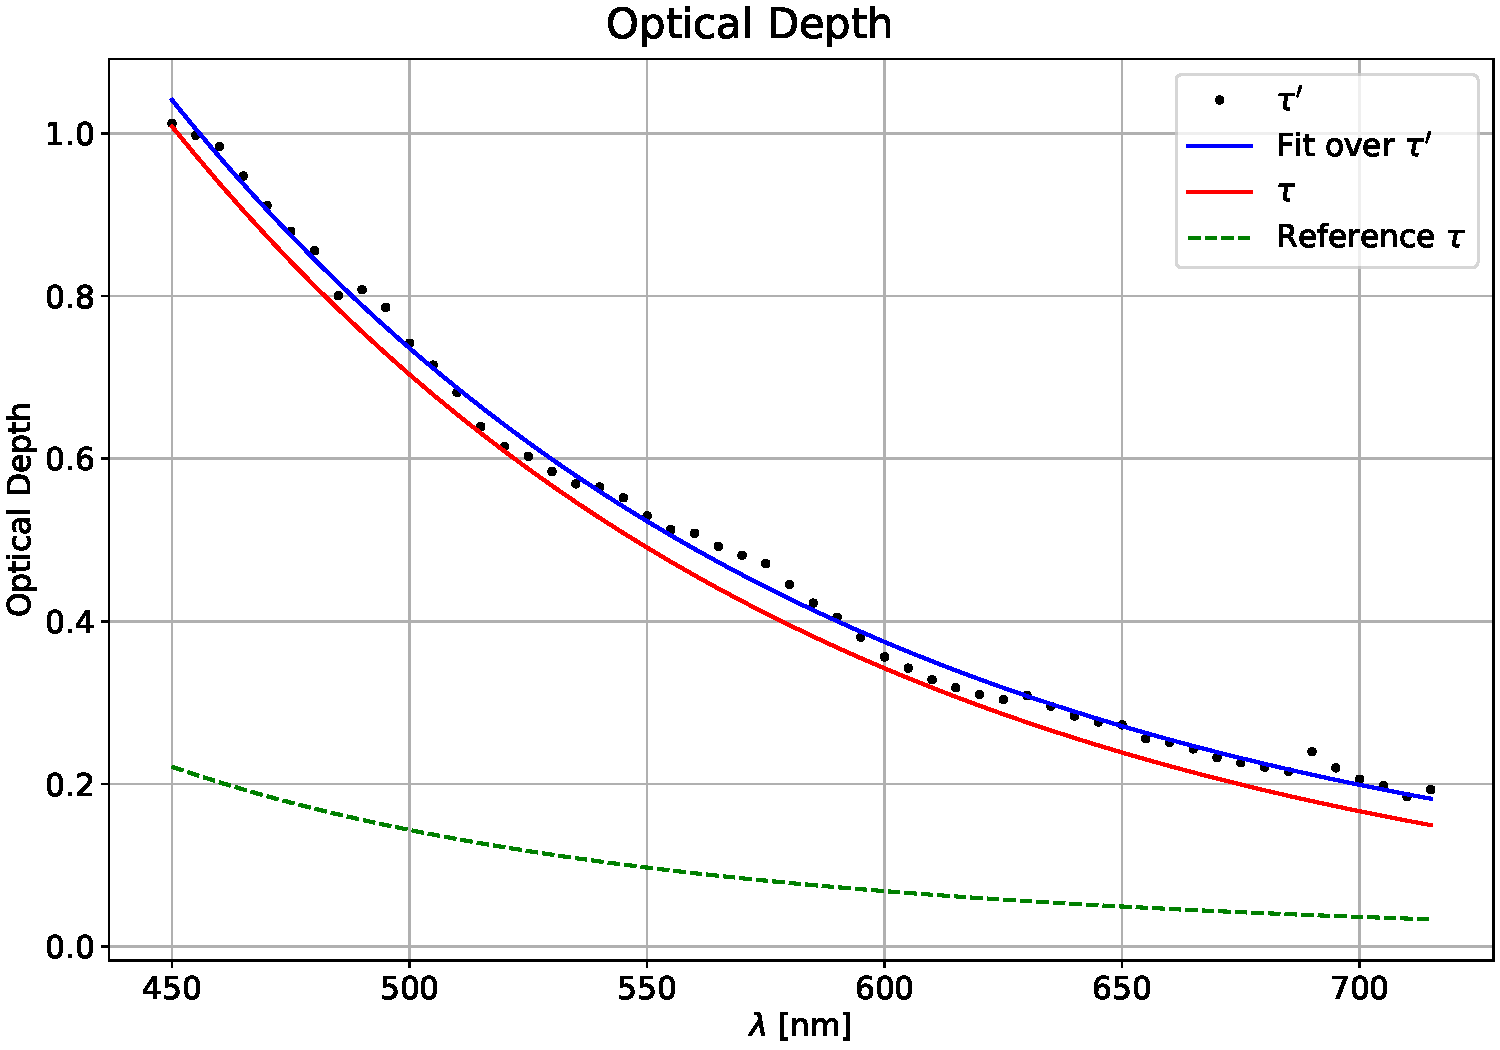
\includegraphics[width=\linewidth]{Opt_depth.pdf}
				\captionof{figure}{Derived optical depth}
				\label{fig:opt_depth}
			\end{Figure}
			\begin{Figure}
				\centering
				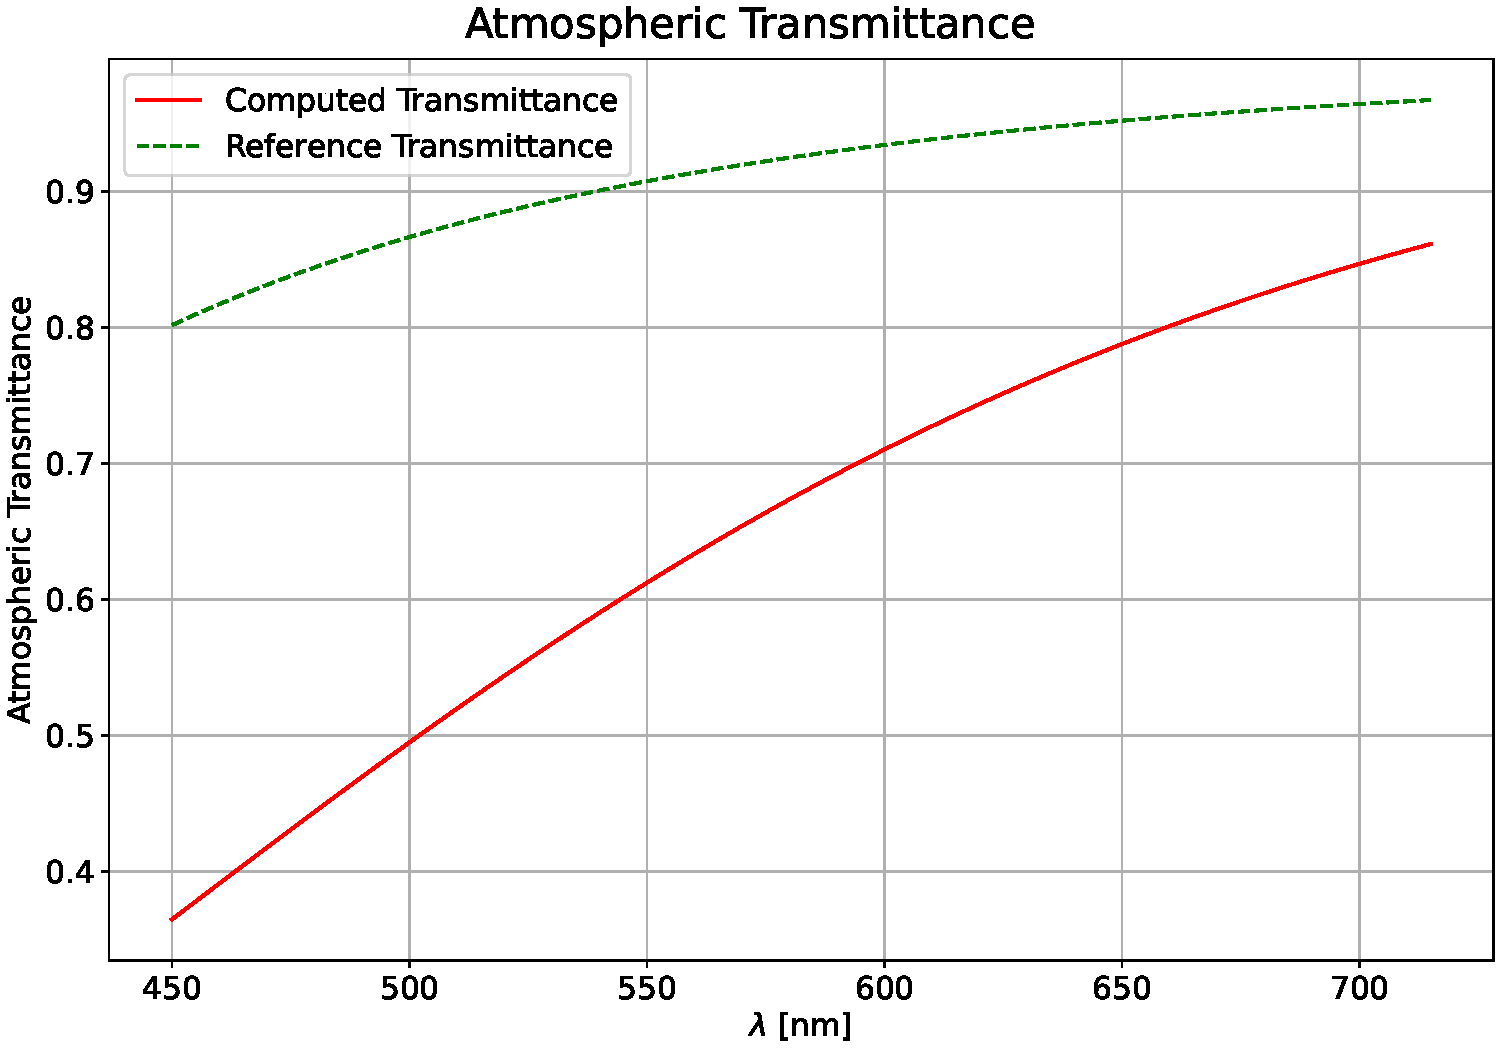
\includegraphics[width=\linewidth]{Atm_trans.pdf}
				\captionof{figure}{Atmospheric transmittance}
				\label{fig:atm_tr}
			\end{Figure}
			It is clear that the atmospheric transmittance found is different from a pure Rayleigh scattering atmosphere. This highlights the presence of phenomena that depend on frequency and/or angle.\\
			
			The problem now is that we can only infer $A_2/A_1$, not the two values singularly.\\
			Since the first observation was the one at lower airmass (thus supposedly better) it was chosen $A_1 = 1$ and, consequently, $A_2 = \frac{t_{exp,1}}{t_{exp,2}} \exp((a_1 - a_2)c)$.\\
		
		\subsection{CCD Response function}
			Taking now the absolute spectrum of Vega as $I(\lambda)$ we can find
			\begin{equation*}
				S_0 = \frac{N_i}{I_{Vega,std} \cdot T_0^{a_i} \cdot t_{exp,i} \cdot A_i}
			\end{equation*}
			The two $S_0$ computed using the two Sirius spectra are very close, at least showing the autoconsistency of this operation. The "true" $S_0$ was then taken then as the smoothed average of the two.
			\begin{Figure}
				\centering
				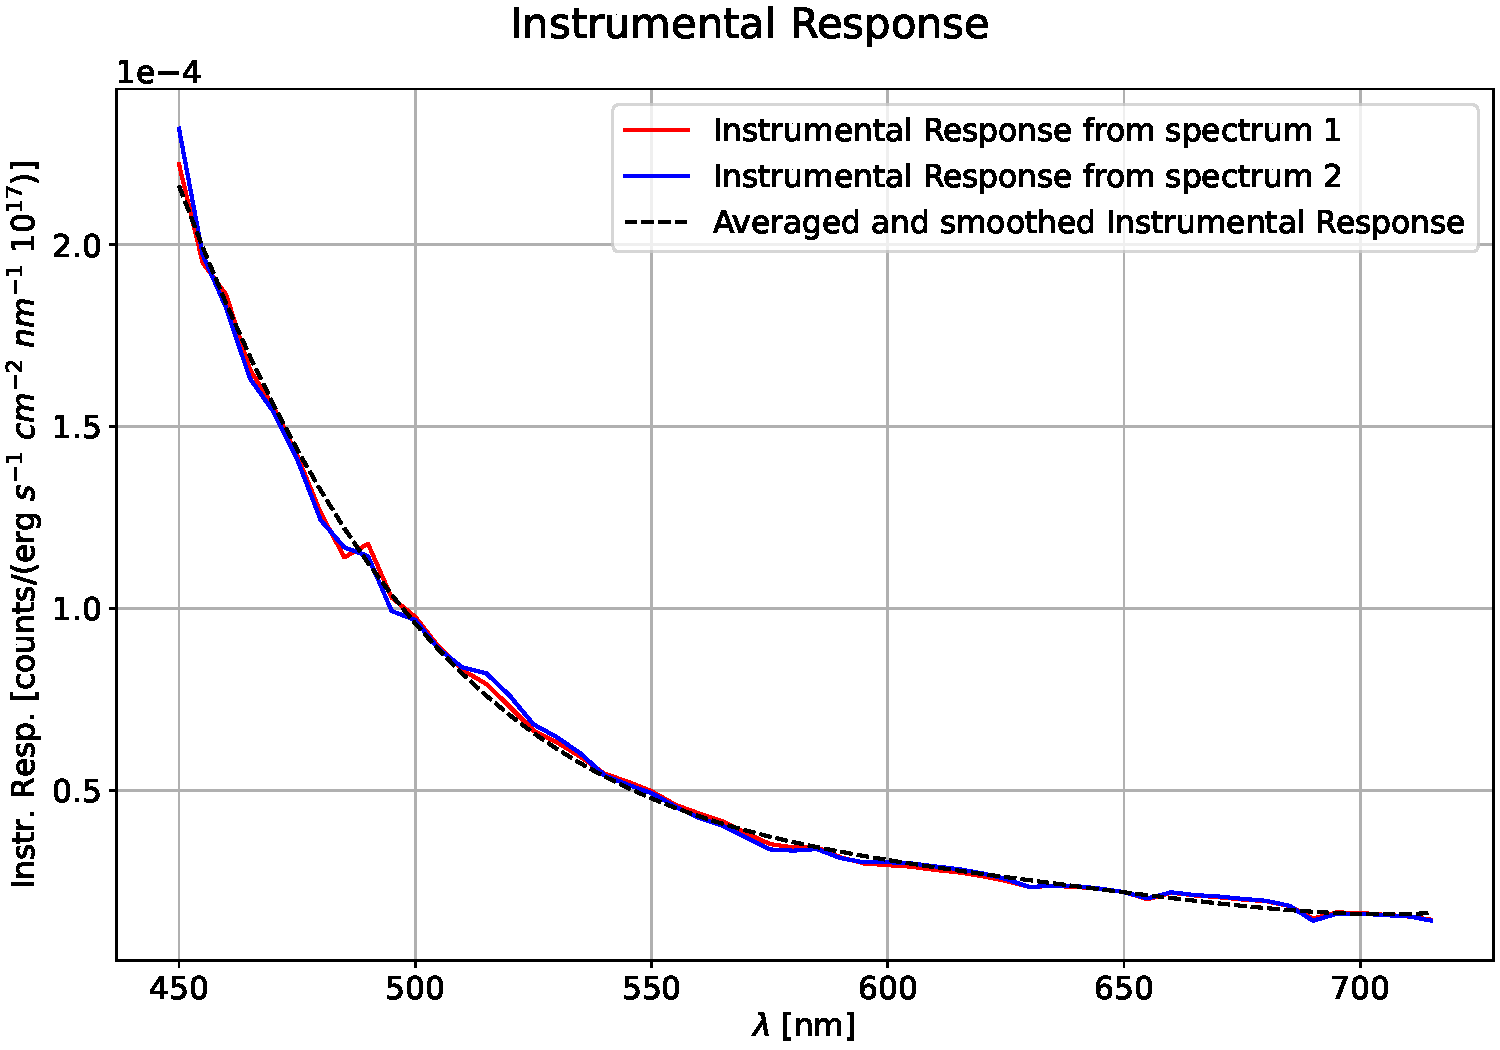
\includegraphics[width=\linewidth]{Instr_resp.pdf}
				\captionof{figure}{Instrumental response}
				\label{fig:instr_re}
			\end{Figure}
			
			\vspace{0.01\textheight}
			
			The total response function at 1 airmass and 1 second exposure can thus be computed as $R_0 = T_0 \cdot S_0$.
			\begin{Figure}
				\centering
				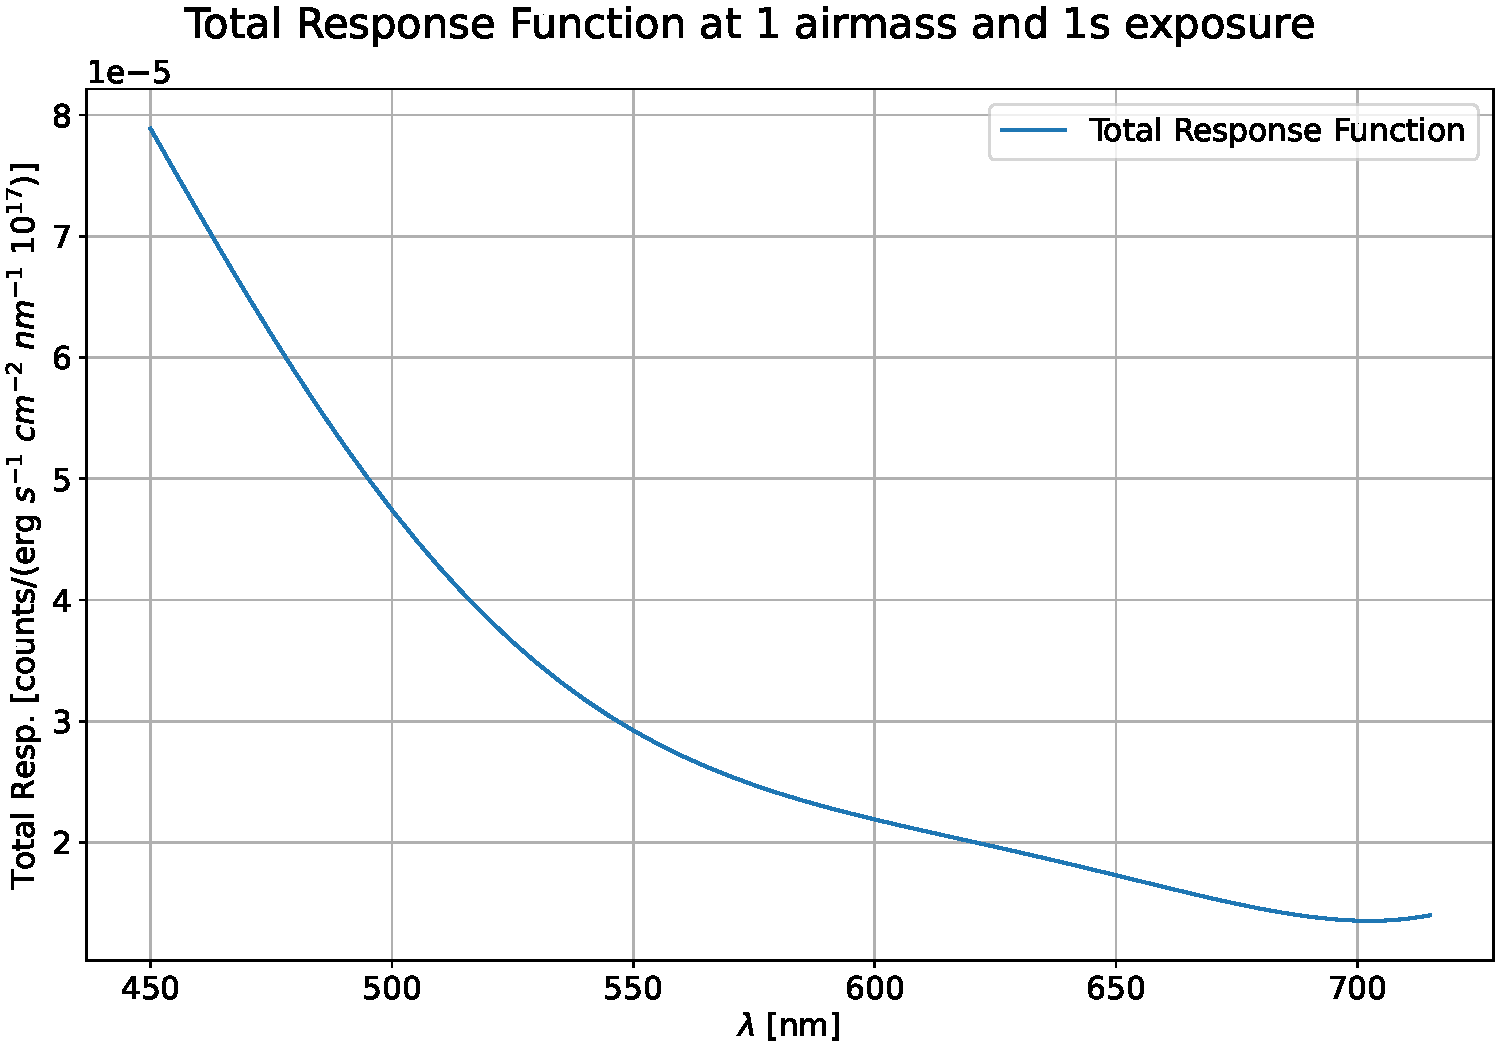
\includegraphics[width=\linewidth]{Tot_resp.pdf}
				\captionof{figure}{Total Response function}
				\label{fig:resp_tot}
			\end{Figure}
		
		\subsection{Further comments}
			It is clear that the results are not accurate. This is mainly due to the many assumptions made, but probably also due to the conditions in which the observations were made.\\
			
			In principle, to get a true absolute calibration, a standard star should have been observed in the same conditions as the two spectra used to compute the atmospheric transmittance. With such an observation the standard spectrum could have been applied directly to the corresponding star, thus getting a more precise $R(t_{exp}, a)$.\\
			
			The plane parallel approximation would also work better at smaller airmasses, so another improvement could be the use of a star nearer to azimuth.
			
	\end{multicols}
	
	\newpage
	\section{Appendix}
		\subsection{Response functions use}
			The response functions computed have limited use.\\
			If the quality was better they could be used to correct the observations made at least during the same hours of the same night.\\
			In general they can be used during observation planning, especially for exposure time setting.\\
			
		\subsection{Sample spectra extraction}
		As an example the spectrum for Polaris is extracted and shown below.
		It can be noted the correct placement of the H$\alpha$ and H$\beta$ line in all spectra showing that the conversion px-nm was successful.\\
		
		\begin{Figure}
			\centering
			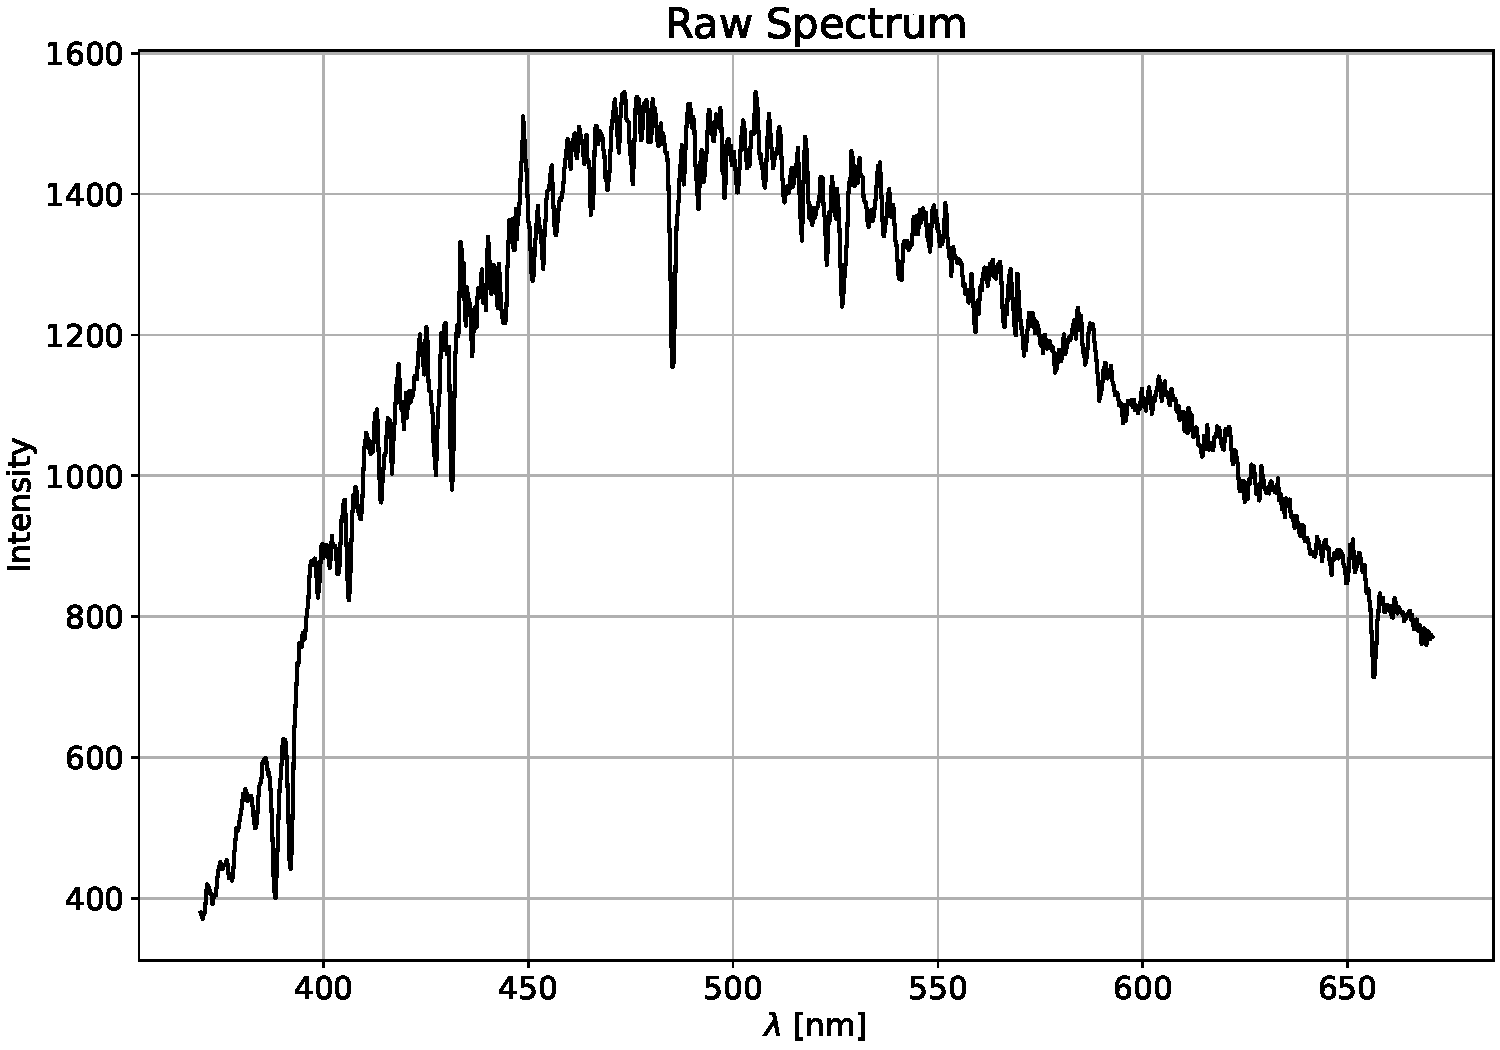
\includegraphics[width=\linewidth]{Polaris_raw.pdf}
			\captionof{figure}{Polaris raw spectrum}
			\label{fig:pol_raw}
		\end{Figure}
		\begin{Figure}
			\centering
			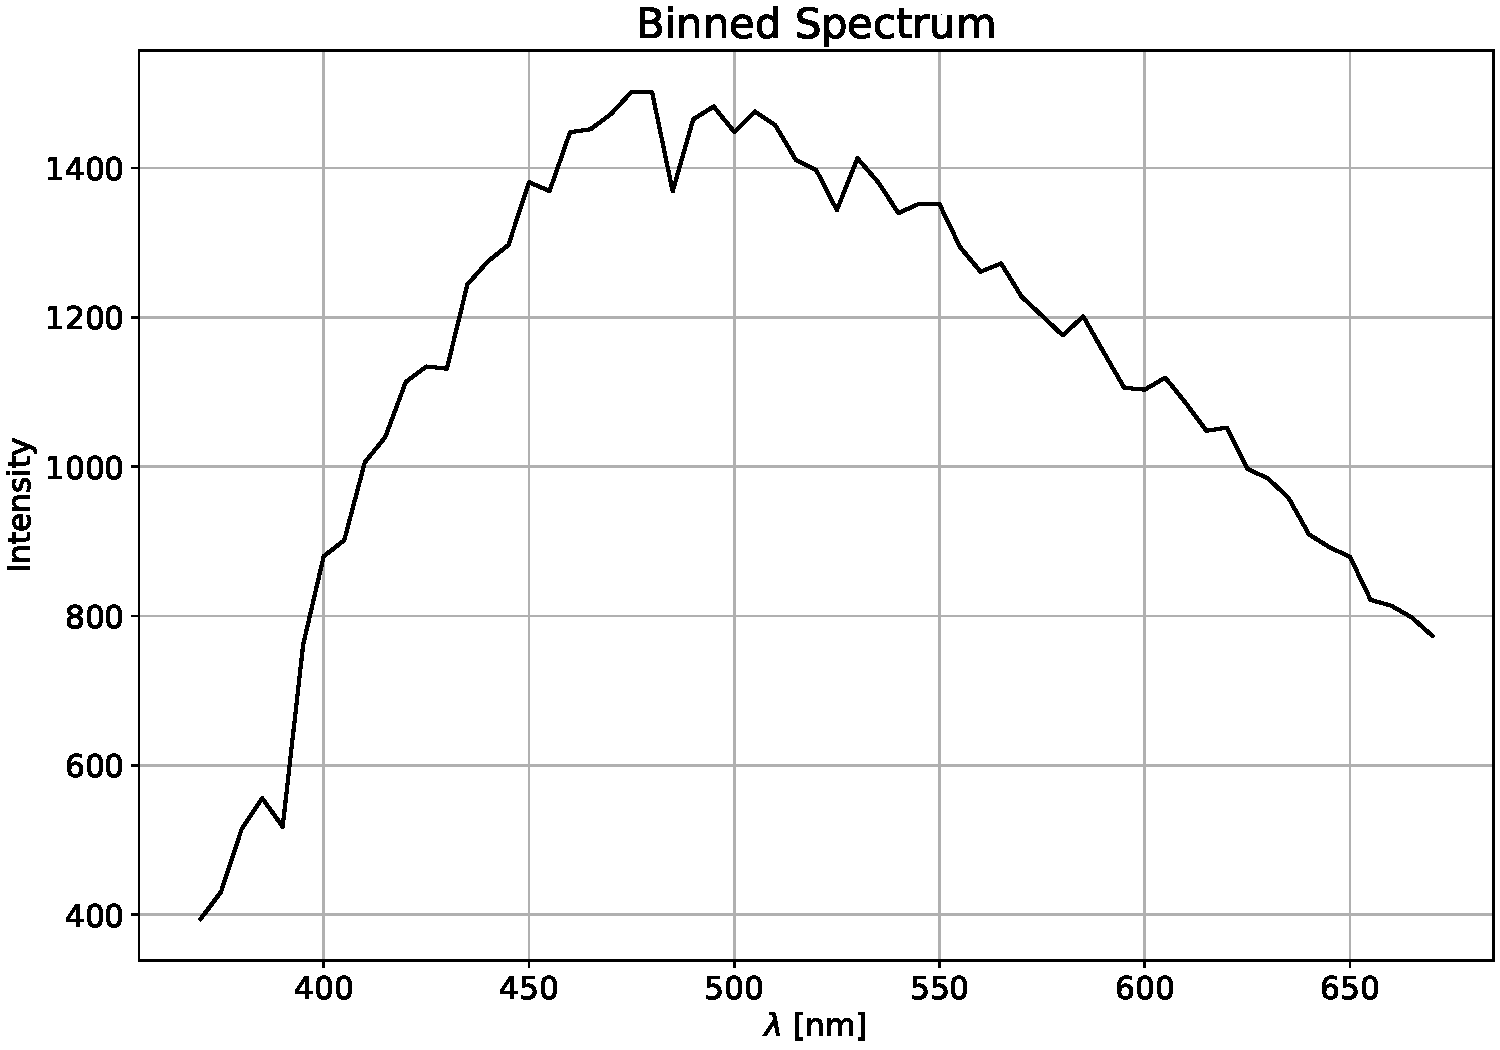
\includegraphics[width=0.95\linewidth]{Polaris_bin.pdf}
			\captionof{figure}{Polaris raw binned spectrum}
			\label{fig:pol_bin}
		\end{Figure}
		\begin{Figure}
			\centering
			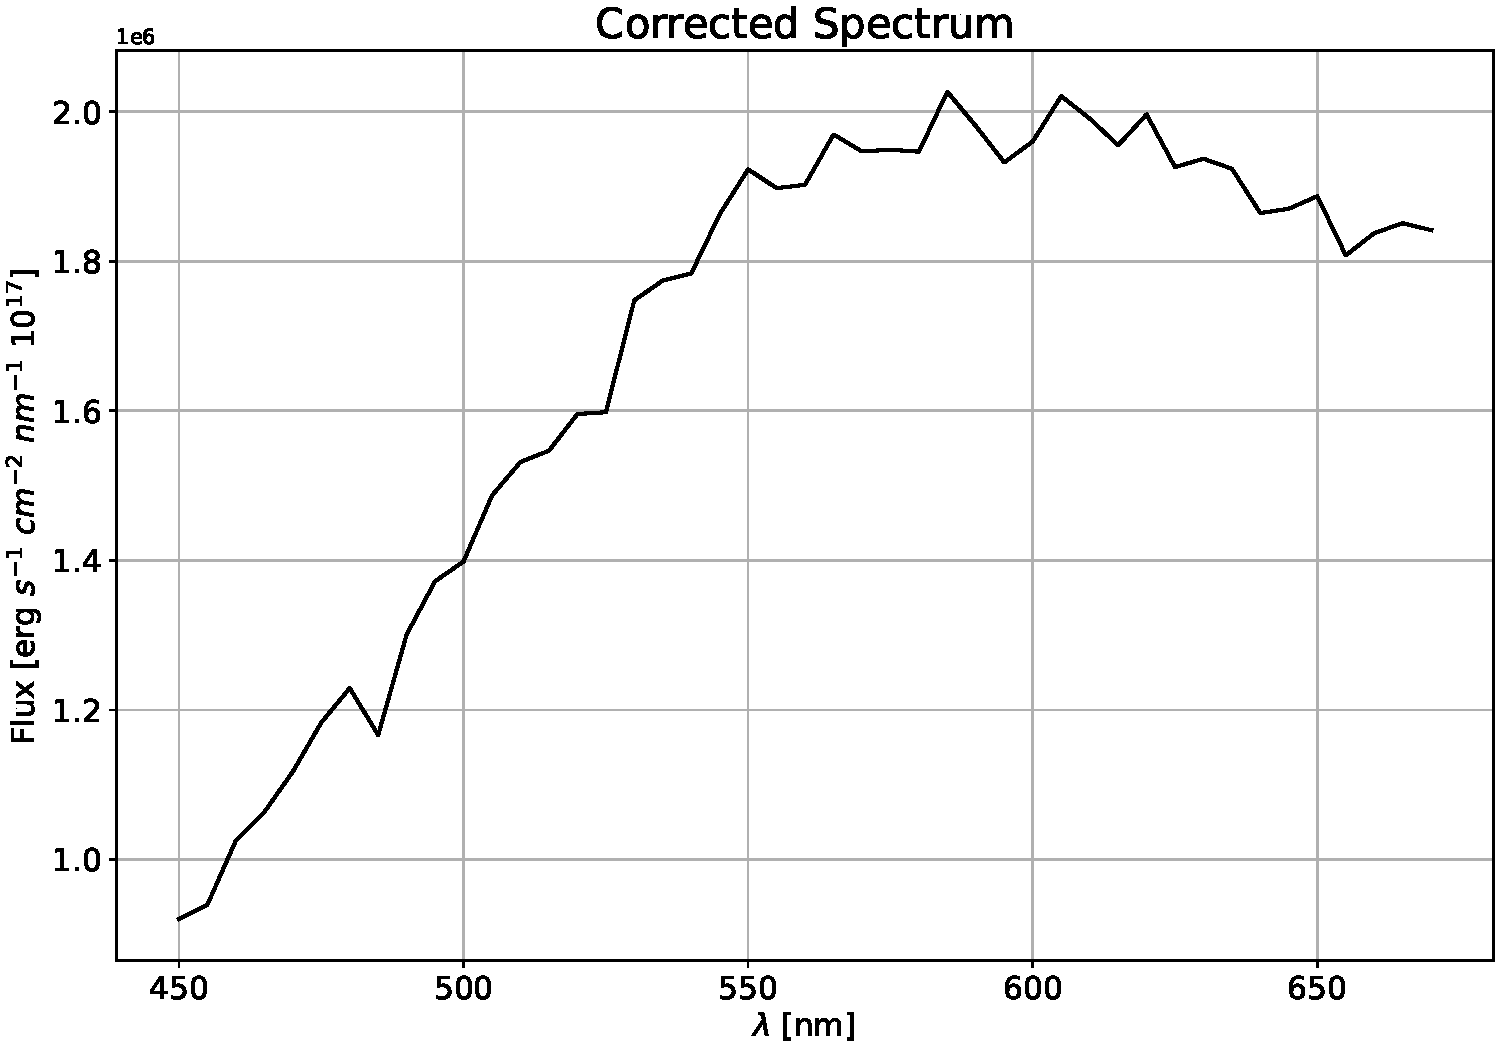
\includegraphics[width=0.95\linewidth]{Polaris_corr.pdf}
			\captionof{figure}{Polaris corrected spectrum}
			\label{fig:pol_corr}
		\end{Figure}
		
\end{document}